% % % % % % % % % % % % % % % % % % % % % % % % % % % % % % % % % % % % % % % %
% IEEE Style - Double columns, 11pt font, letterpaper
\documentclass[journal, twocolumn, final,11pt,letterpaper]{IEEEtran}	

% Include Latex Packages
\usepackage{etex}	% This package enables the use of many packages

% % Page styles
\usepackage{setspace}	% line spacing package
\doublespacing			% use double spacing
%\linespread{1.6}		% Use linespread to fine tune line spacing, not recommended


% % Figures
\usepackage{float}		% improves interface for floating objects
\usepackage{subfig}		% enables subfloat
\usepackage{graphicx}	% more image type support
\usepackage{circuitikz}
\usepackage{epstopdf}	% automatically convert included eps files to pdf
\usepackage{tikz}
%\usepackage{listings}
\usepackage{color}
\definecolor{dkgreen}{rgb}{0,0.6,0}
\definecolor{gray}{rgb}{0.5,0.5,0.5}
\definecolor{mauve}{rgb}{0.58,0,0.82}

\lstset{frame=tb,
	language=Verilog,
	aboveskip=3mm,
	belowskip=3mm,
	showstringspaces=false,
	columns=flexible,
	basicstyle={\small\ttfamily},
	numbers=none,
	numberstyle=\tiny\color{gray},
	keywordstyle=\color{blue},
	commentstyle=\color{dkgreen},
	stringstyle=\color{mauve},
	breaklines=true,
	breakatwhitespace=true,
	tabsize=3
}
\usetikzlibrary{matrix,calc}
\usetikzlibrary{shapes}

\newcommand*{\circled}[2][red]{
	\tikz[baseline=(char.base)]{
		\node[shape=ellipse,inner sep=1pt,
		draw=#1,
		] (char) {#2};}
}

%isolated term
%#1 - Optional. Space between node and grouping line. Default=0
%#2 - node
%#3 - filling color
\newcommand{\implicantsol}[3][0]{
	\draw[rounded corners=3pt, fill=#3, opacity=0.3] ($(#2.north west)+(135:#1)$) rectangle ($(#2.south east)+(-45:#1)$);
}


%internal group
%#1 - Optional. Space between node and grouping line. Default=0
%#2 - top left node
%#3 - bottom right node
%#4 - filling color
\newcommand{\implicant}[4][0]{
	\draw[rounded corners=3pt, fill=#4, opacity=0.3] ($(#2.north west)+(135:#1)$) rectangle ($(#3.south east)+(-45:#1)$);
}

%group lateral borders
%#1 - Optional. Space between node and grouping line. Default=0
%#2 - top left node
%#3 - bottom right node
%#4 - filling color
\newcommand{\implicantcostats}[4][0]{
	\draw[rounded corners=3pt, fill=#4, opacity=0.3] ($(rf.east |- #2.north)+(90:#1)$)-| ($(#2.east)+(0:#1)$) |- ($(rf.east |- #3.south)+(-90:#1)$);
	\draw[rounded corners=3pt, fill=#4, opacity=0.3] ($(cf.west |- #2.north)+(90:#1)$) -| ($(#3.west)+(180:#1)$) |- ($(cf.west |- #3.south)+(-90:#1)$);
}

%group top-bottom borders
%#1 - Optional. Space between node and grouping line. Default=0
%#2 - top left node
%#3 - bottom right node
%#4 - filling color
\newcommand{\implicantdaltbaix}[4][0]{
	\draw[rounded corners=3pt, fill=#4, opacity=0.3] ($(cf.south -| #2.west)+(180:#1)$) |- ($(#2.south)+(-90:#1)$) -| ($(cf.south -| #3.east)+(0:#1)$);
	\draw[rounded corners=3pt, fill=#4, opacity=0.3] ($(rf.north -| #2.west)+(180:#1)$) |- ($(#3.north)+(90:#1)$) -| ($(rf.north -| #3.east)+(0:#1)$);
}

%group corners
%#1 - Optional. Space between node and grouping line. Default=0
%#2 - filling color
\newcommand{\implicantcantons}[2][0]{
	\draw[rounded corners=3pt, opacity=.3] ($(rf.east |- 0.south)+(-90:#1)$) -| ($(0.east |- cf.south)+(0:#1)$);
	\draw[rounded corners=3pt, opacity=.3] ($(rf.east |- 8.north)+(90:#1)$) -| ($(8.east |- rf.north)+(0:#1)$);
	\draw[rounded corners=3pt, opacity=.3] ($(cf.west |- 2.south)+(-90:#1)$) -| ($(2.west |- cf.south)+(180:#1)$);
	\draw[rounded corners=3pt, opacity=.3] ($(cf.west |- 10.north)+(90:#1)$) -| ($(10.west |- rf.north)+(180:#1)$);
	\fill[rounded corners=3pt, fill=#2, opacity=.3] ($(rf.east |- 0.south)+(-90:#1)$) -|  ($(0.east |- cf.south)+(0:#1)$) [sharp corners] ($(rf.east |- 0.south)+(-90:#1)$) |-  ($(0.east |- cf.south)+(0:#1)$) ;
	\fill[rounded corners=3pt, fill=#2, opacity=.3] ($(rf.east |- 8.north)+(90:#1)$) -| ($(8.east |- rf.north)+(0:#1)$) [sharp corners] ($(rf.east |- 8.north)+(90:#1)$) |- ($(8.east |- rf.north)+(0:#1)$) ;
	\fill[rounded corners=3pt, fill=#2, opacity=.3] ($(cf.west |- 2.south)+(-90:#1)$) -| ($(2.west |- cf.south)+(180:#1)$) [sharp corners]($(cf.west |- 2.south)+(-90:#1)$) |- ($(2.west |- cf.south)+(180:#1)$) ;
	\fill[rounded corners=3pt, fill=#2, opacity=.3] ($(cf.west |- 10.north)+(90:#1)$) -| ($(10.west |- rf.north)+(180:#1)$) [sharp corners] ($(cf.west |- 10.north)+(90:#1)$) |- ($(10.west |- rf.north)+(180:#1)$) ;
}

%Empty Karnaugh map 4x4
\newenvironment{Karnaugh}%
{
	\begin{tikzpicture}[baseline=(current bounding box.north),scale=0.8]
	\draw (0,0) grid (4,4);
	\draw (0,4) -- node [pos=0.9,above right,anchor=south west] {C1C0} node [pos=0.9,below left,anchor=north east] {EQ} ++(135:1);
	%
	\matrix (mapa) [matrix of nodes,
	column sep={0.8cm,between origins},
	row sep={0.8cm,between origins},
	every node/.style={minimum size=0.3mm},
	anchor=8.center,
	ampersand replacement=\&] at (0.5,0.5)
	{
		\& |(c00)| 00         \& |(c01)| 01         \& |(c11)| 11         \& |(c10)| 10         \& |(cf)| \phantom{00} \\
		|(r00)| 00             \& |(0)|  \phantom{0} \& |(1)|  \phantom{0} \& |(3)|  \phantom{0} \& |(2)|  \phantom{0} \&                     \\
		|(r01)| 01             \& |(4)|  \phantom{0} \& |(5)|  \phantom{0} \& |(7)|  \phantom{0} \& |(6)|  \phantom{0} \&                     \\
		|(r11)| 11             \& |(12)| \phantom{0} \& |(13)| \phantom{0} \& |(15)| \phantom{0} \& |(14)| \phantom{0} \&                     \\
		|(r10)| 10             \& |(8)|  \phantom{0} \& |(9)|  \phantom{0} \& |(11)| \phantom{0} \& |(10)| \phantom{0} \&                     \\
		|(rf) | \phantom{00}   \&                    \&                    \&                    \&                    \&                     \\
	};
}%
{
	\end{tikzpicture}
}

%Empty Karnaugh map 2x4
\newenvironment{Karnaughvuit}%
{
	\begin{tikzpicture}[baseline=(current bounding box.north),scale=0.8]
	\draw (0,0) grid (4,2);
	\draw (0,2) -- node [pos=0.7,above right,anchor=south west] {LA/LB} node [pos=0.6,below left,anchor=north east] {S} ++(120:1);
	%
	\matrix (mapa) [matrix of nodes,
	column sep={0.8cm,between origins},
	row sep={0.8cm,between origins},
	every node/.style={minimum size=0.3mm},
	anchor=4.center,
	ampersand replacement=\&] at (0.5,0.5)
	{
		\& |(c00)| 00         \& |(c01)| 01         \& |(c11)| 11         \& |(c10)| 10         \& |(cf)| \phantom{00} \\
		|(r00)| 0             \& |(0)|  \phantom{0} \& |(1)|  \phantom{0} \& |(3)|  \phantom{0} \& |(2)|  \phantom{0} \&                     \\
		|(r01)| 1             \& |(4)|  \phantom{0} \& |(5)|  \phantom{0} \& |(7)|  \phantom{0} \& |(6)|  \phantom{0} \&                     \\
		|(rf) | \phantom{00}  \&                    \&                    \&                    \&                    \&                     \\
	};
}%
{
	\end{tikzpicture}
}

%Empty Karnaugh map 2x2
\newenvironment{Karnaughquatre}%
{
	\begin{tikzpicture}[baseline=(current bounding box.north),scale=0.8]
	\draw (0,0) grid (2,2);
	\draw (0,2) -- node [pos=0.7,above right,anchor=south west] {b} node [pos=0.7,below left,anchor=north east] {a} ++(135:1);
	%
	\matrix (mapa) [matrix of nodes,
	column sep={0.8cm,between origins},
	row sep={0.8cm,between origins},
	every node/.style={minimum size=0.3mm},
	anchor=2.center,
	ampersand replacement=\&] at (0.5,0.5)
	{
		\& |(c00)| 0          \& |(c01)| 1  \\
		|(r00)| 0 \& |(0)|  \phantom{0} \& |(1)|  \phantom{0} \\
		|(r01)| 1 \& |(2)|  \phantom{0} \& |(3)|  \phantom{0} \\
	};
}%
{
	\end{tikzpicture}
}

%Defines 8 or 16 values (0,1,X)
\newcommand{\contingut}[1]{%
	\foreach \x [count=\xi from 0]  in {#1}
	\path (\xi) node {\x};
}

%Places 1 in listed positions
\newcommand{\minterms}[1]{%
	\foreach \x in {#1}
	\path (\x) node {1};
}

%Places 0 in listed positions
\newcommand{\maxterms}[1]{%
	\foreach \x in {#1}
	\path (\x) node {0};
}

%Places X in listed positions
\newcommand{\indeterminats}[1]{%
	\foreach \x in {#1}
	\path (\x) node {X};
}



% % Maths
\usepackage[cmex10]{amsmath}	% Maths
\usepackage{amsfonts,amssymb} 	% maths symbols

% % Tables
\usepackage{booktabs}  % professional-looking tables
\usepackage{multicol} %used for getting multicolumn without page-break
\usepackage{multirow}	% multi-row tables
\usepackage{array}		% define column format of a table

% % Others
\usepackage{caption}	%Customising captions in floating environments
%\usepackage{abstract}
\usepackage{cite}		% cite multiple
\usepackage{fixltx2e}	%added by pilawa, preventing figure* to get ahead of regular figures.
\usepackage{url}		% url display

% %
\hyphenation{op-tical net-works semi-conduc-tor}	% correct bad hyphenation here
\providecommand{\e}[1]{\ensuremath{\times 10^{#1}}}		% use use \e{2} for scientific number expression


% % Optional packages that might be useful
%\usepackage{epsf}		% eps fix
%\usepackage{verbatim}	% verbatim text are not interpreted by the compiler 
%\numberwithin{equation}{section}	% number equation according to section
%\usepackage{xfrac}		% slanted fraction
%\usepackage{pgfplots}	% plot graph
%\usepackage{tikz,pgfplots} % plot graph
%\usepackage{endnotes}	% endnotes


% Title of Document
\title{ECE385 Experiment \#5
	}
\author{
\IEEEauthorblockN{Eric Meyers, Ryan Helsdingen}\\
\IEEEauthorblockA{Section ABG; TAs: Ben Delay, Shuo Liu \\
February 24th, 2016 \\
emeyer7, helsdin2}}
% % % % % % % % % % % % % % % % % % % % % % % % % % % % % % % % % % % % % % % 
\begin{document}
	
%SECTION : Formatting and Title
\maketitle
\singlespacing

%SECTION 1 - Introduction - Eric
\section{Introduction}
The purpose of this lab was to design and construct a 2s compliment 8-bit multiplier that uses a shift-and-add algorithm. The user will input their desired multiplicand and multiplier into switches and these will be stored in two shift registers (A and B). The multiplier is built upon a control unit with a state machine, so once the "run" button is pressed, the machine will cycle through multiple states and output the value in the combined 16-bit value "AB".

%SECTION 2 - 8-bit Multiplication Example - Ryan
\section{8-bit Multiplication Example}
Table \ref{tab:table1} shows each step of the multiplication process given inputs Multiplier B=7 and Multiplicand S=-59.  The result is -413 in decimal and 1111 1110 0110 0011 in binary.  As you can see, bolded at the bottom of Table \ref{tab:table1} is the expected result loaded into A and B. Shift functions occur eight times, right-shifting the bit.  Add functions occur before each shift and only if the previous M bit is equal to 1.  During an add function, S gets added to A.  The only exception is before the eighth shift which would be a subtract function rather than an add function.  S would get subtracted from A.  This exception, as you can see, is not needed for this example.


\begin{table}[htbp]
	\centering
	\caption{Reworked 8-bit Multiplication Problem. }
	\begin{tabular}{ccccc}	% ccccccc indicates 7 center aligned columns
		\toprule	% top separator
		Function & X & A & B & M \\
		\midrule
		Clr\_A\_Ld\_B & 0 & 0000 0000 & 0000 0111 & 1 \\ 
		ADD (1)    & 1 & 1100 0101 & 0000 0111 & 1 \\
		SHIFT (1)  & 1 & 1110 0010 & 1000 0011 & 1 \\

		ADD (2)    & 1 & 1010 0111 & 1000 0011 & 1 \\
		SHIFT (2)  & 1 & 1101 0011 & 1100 0001 & 1 \\		
		ADD (3)    & 1 & 1001 1000 & 1100 0001 & 1 \\
		SHIFT (3)  & 1 & 1100 1100 & 0110 0000 & 0 \\		
		SHIFT (4)  & 1 & 1110 0110 & 0011 0000 & 0 \\		
		SHIFT (5)  & 1 & 1111 0011 & 0001 1000 & 0 \\		
		SHIFT (6)  & 1 & 1111 1001 & 1000 1100 & 0 \\		
		SHIFT (7)  & 1 & 1111 1100 & 1100 0110 & 0 \\		
		SHIFT (8)  & 1 & \textbf{1111 1110} & \textbf{0110 0011} & 1 \\
		\bottomrule	% bottom separator
	\end{tabular}%
	\label{tab:table1}	% this is the label given to the table that can be referenced using \ref{tab:Exp1Part1_7}
\end{table}%


%SECTION 3 - Description of Circuit - Eric
\section{Description of Circuit}
The purpose of the 8-bit multiplier is to take two 8-bit user-defined words, multiply them together and place the resulting product in the two combined registers. \\

Initially both storage registers will begin with 00000000 loaded into them. On the Altera Board, the operator will control the last eight general purpose switches to indicate what the word they wish to load is, then press the "Clear\_A\_Load\_B" push button to the right. This will then take the switch values and load them into Register B. Therefore after this operation is performed, A will still contain 00000000, and B will contain XXXXXXXX (X being the value the user defines).\\

Then once the user indicates the multiplier (Register B), they will then indicate the multiplicand by changing the order of the eight switches. Once this is done, then the user will press the "Run" switch and the control unit will cycle through all states within the FSM and come to a halt. The product of the two values will be displayed in register AB(concatenated A + B) and the X bit will be displayed on the green LED next to the HEX values. \\

The FSM is a part of the control unit and will be explained below and the "X-bit" will also be described in detail below. 

%SECTION 4 - Purpose of Modules - Eric
\section{Purpose of Modules}
Please refer to Figure \ref{fig:block-diagram} to understand the how each module interacts with one another. The multiplier is broken down into four primary modules as listed below:
\begin{itemize}
	\item Shift Register 
	\item Full Adder/Subtractor
	\item Control Unit 
	\item X Register 
\end{itemize} 

The first of these modules is the shift register and it's purpose is to store the contents of each 8-bit word the user specifies. The concatenation of the two registers together (AB) contains the 16-bit product of the multiplication. The shift register shifts right when enabled by the control unit, pushing the least significant bit out through its "shift\_out" output. The data also is parallel loaded in through its input in the module and has parallel outputs used to display on LEDs on the Altera Board. \\

The next module is the Full Adder/Subtractor which essentially does exactly what it states: both adds and subtracts (depending on the control unit). The inputs are 16 data bits (8 bits for A and 8 bits for B) and a "subtract" bit which indicates whether or not subtraction must be performed.\\

Because subtraction is adding the 2s complement of a number, the team decided to use a trick learned back in Lab 3. To get the 2s complement, one must flip all of the bits and add one. To conditionally flip all of the bits, the team used an XOR gate with inputs of B and the "subtract" bit. This is because if the "subtract" bit is high, then the B value must be flipped, and if it is low then it stays the same. Then this logic value must be fed into the nine inputs of the full adders along with the "subtract" bit on the first full adder. Please reference Figure \ref{fig:full-adder-subtractor-diagram} to get a better understanding of this. \\

This setup will take the 2s complement of the number and add it to the A value if the "subtract" bit is high, but if the "subtract" bit is low then it will simply regularly add the two A and B values. \\

The next module is the Control Unit which dictates how the Finite State Machine operates and how the entire circuit functions. This unit takes in 3 inputs (Run, Reset, and Clear\_A\_Load\_B) that are designated by the operator. These inputs then determine the outputs of the control unit which are Load, Shift, Add, and Shift. These four outputs are determined by the Finite State Machine described in "Section V: State Diagram".\\

 Essentially, the outputs are telling each module if they are in use or not. So for example, if the multiplier needs to perform an "Add" or "Subtract" operation, it will output a high value on the respective output and this will be then fed into the proper module which will then be activated. \\

Last but not least is the "X Register" Module which contains the status of the "X" bit. The "X" bit is essentially the most significant bit in the A register. This register tells whether the result of the multiplication is positive or negative and is mainly used to view the output of the multiplication on the Altera Board by feeding it into a green LED to see its status. 

%SECTION 5 - State Diagram of FSM - Ryan
\section{State Diagram}
RYAN SECTION

%SECTION 6 - Schematic/Block Diagram -Eric
\section{Schematic/Block Diagram}
Please refer to "Section X : Figures" of this document to view the Schematic/Block Diagrams. Figure \ref{fig:full-multiplier-diagram} displays the entire block diagram of the multiplier, with block labels and interconnections. The multiplier, as stated before is broken down into several modules. Those modules are as follows with the figure references aside them:
\begin{itemize}
	\item Shift Register - Figure \ref{fig:shift-register-diagram}
	\item Full Adder/Subtractor - Figure \ref{fig:full-adder-subtractor-diagram}
	\item Control Unit - Figure \ref{fig:top-half-control} (Top Half Only)
	\item Control Unit - Figure \ref{fig:bottom-half-control} (Bottom Half Only)
	\item X Register - Figure \ref{fig:x-ff-diagram}
\end{itemize}

%SECTION 7 - Pre-Lab Simulation Waveforms -Eric
\section{Pre-Lab Simulation Waveforms}
Please refer to "Section X : Figures" of this document to view the Pre-Lab Simulation Waveforms. There was a total of four simulations performed. All options were explored on this multiplier and the following inputs were used: 
\begin{itemize}
	\item \textbf{+}7 * \textbf{-}59 - (Figure \ref{fig:simulation1})
	\item \textbf{-}7 * \textbf{+}59 - (Figure \ref{fig:simulation2t})
	\item \textbf{+}7 * \textbf{+}59 - (Figure \ref{fig:simulation3})
	\item \textbf{-}7 * \textbf{-}59  - (Figure \ref{fig:simulation4})
\end{itemize}
%SECTION 8 - Post Lab -Ryan
\section{Post Lab}
1)  Refer to the Design Resources and Statistics in IQT.30-32 and complete
the following design statistics table.\\

These numbers are shown below in Table \ref{tab:lab5-statistics} .

\begin{table}[htbp]
	\centering
	\caption{Reworked 8-bit Multiplication Problem. }
	\begin{tabular}{c|c}	% ccccccc indicates 7 center aligned columns
		\toprule	% top separator
		LUT & 95\\
		DSP & 0\\
		Memory (BRAM) & 0\\
		Flip-Flop & 0\\
		Frequency & 239.52 MHz\\
		Static Power & 98.52 mW\\
		Dynamic Power & 0 mW\\
		Total Power & 147.8 mW\\
	
		\bottomrule	% bottom separator
	\end{tabular}%
	\label{tab:table2}	% this is the label given to the table that can be referenced using \ref{tab:Exp1Part1_7}
\end{table}%

Come up with a few ideas on how you might optimize your design to decrease the total gate count and/or to increase maximum frequency by changing your code for the design.\\

\textit{Answer:} 

%SECTION 9 - Conclusion - Ryan
\section{Conclusion}
In this lab, the team was able to successfully program and test a working multiplier on the DE2 FPGA board.  

\clearpage
\onecolumn
%SECTION 10: Figures
\section{Figures}

\begin{figure} [htbp]
	\centering
	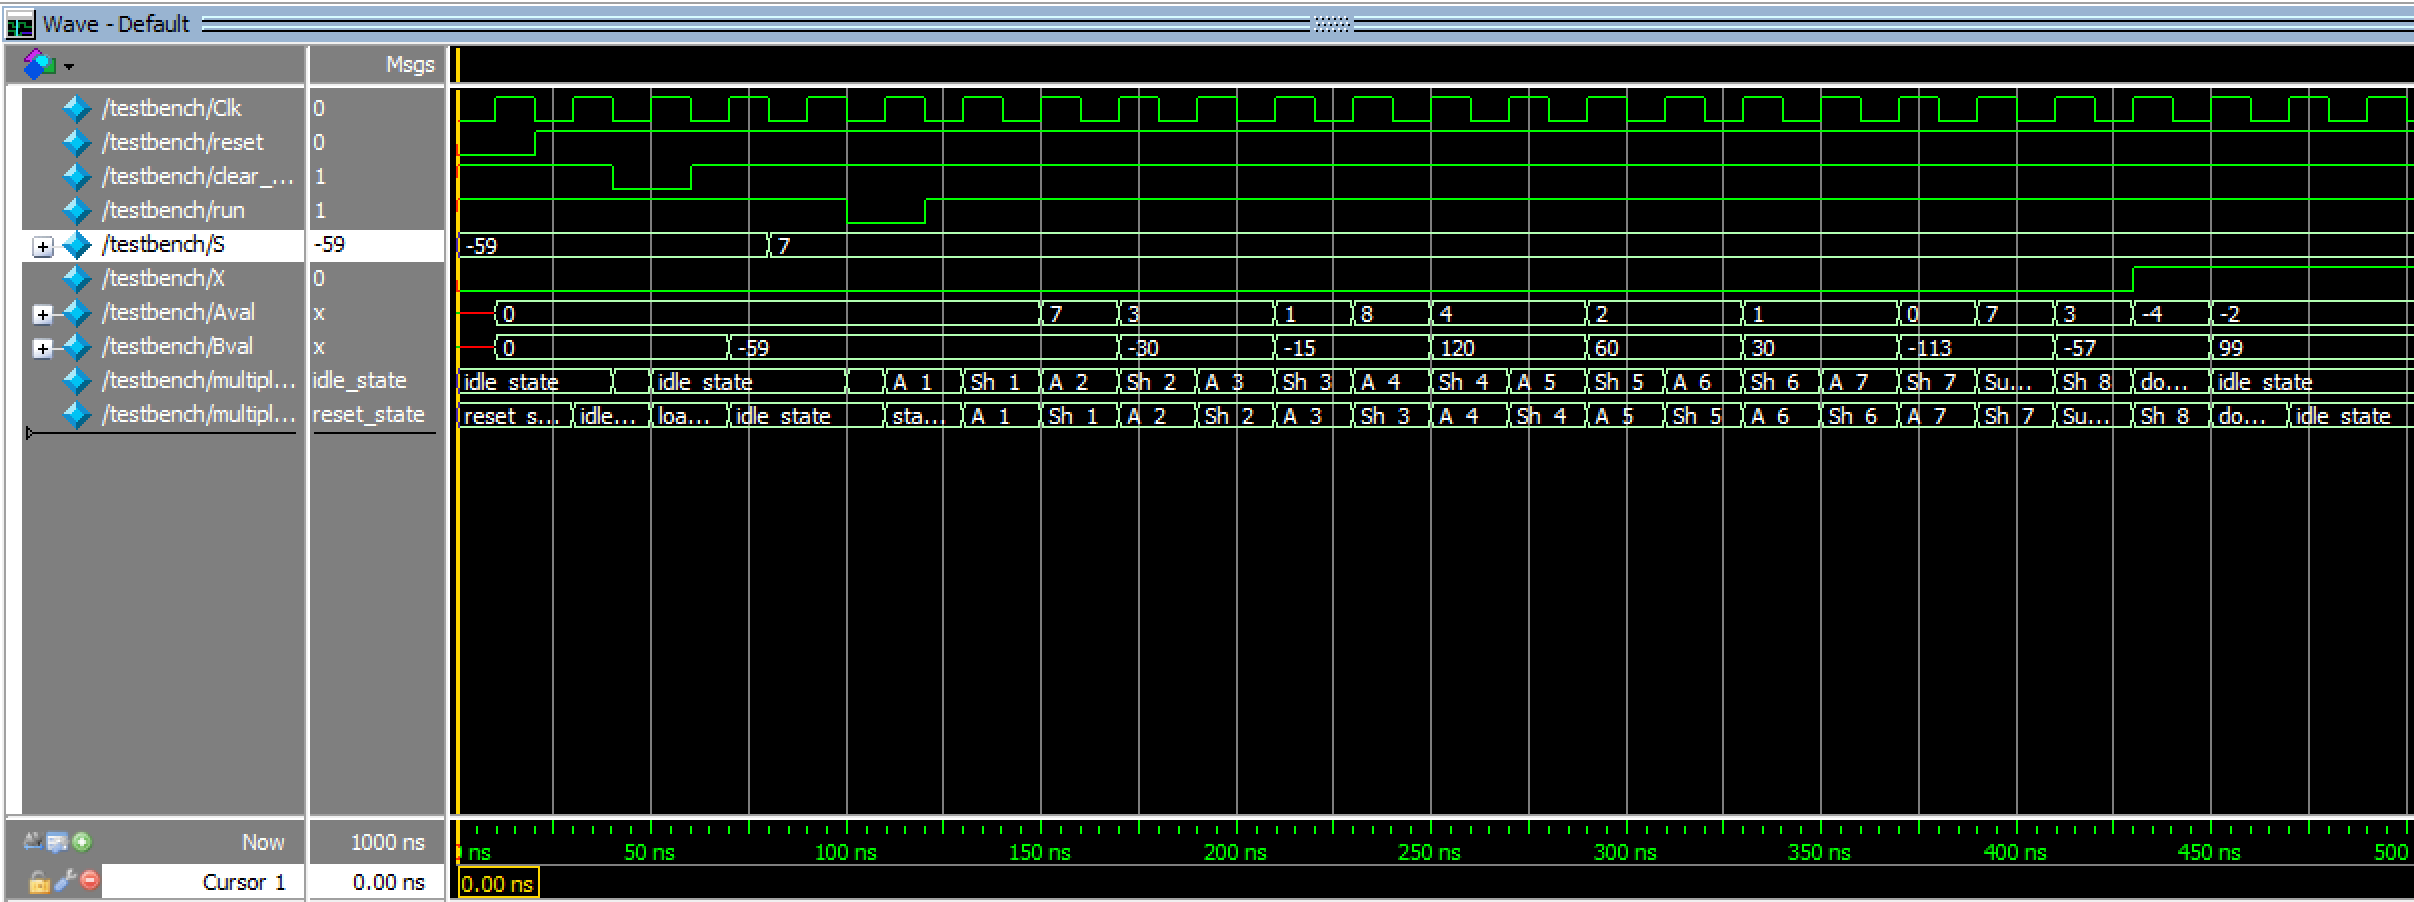
\includegraphics[scale=0.4]{simulation1.png}
	\caption{ModelSim Simulation Output (+7 * -59)\label{fig:simulation1}}
\end{figure}

\begin{figure} [htbp]
	\centering
	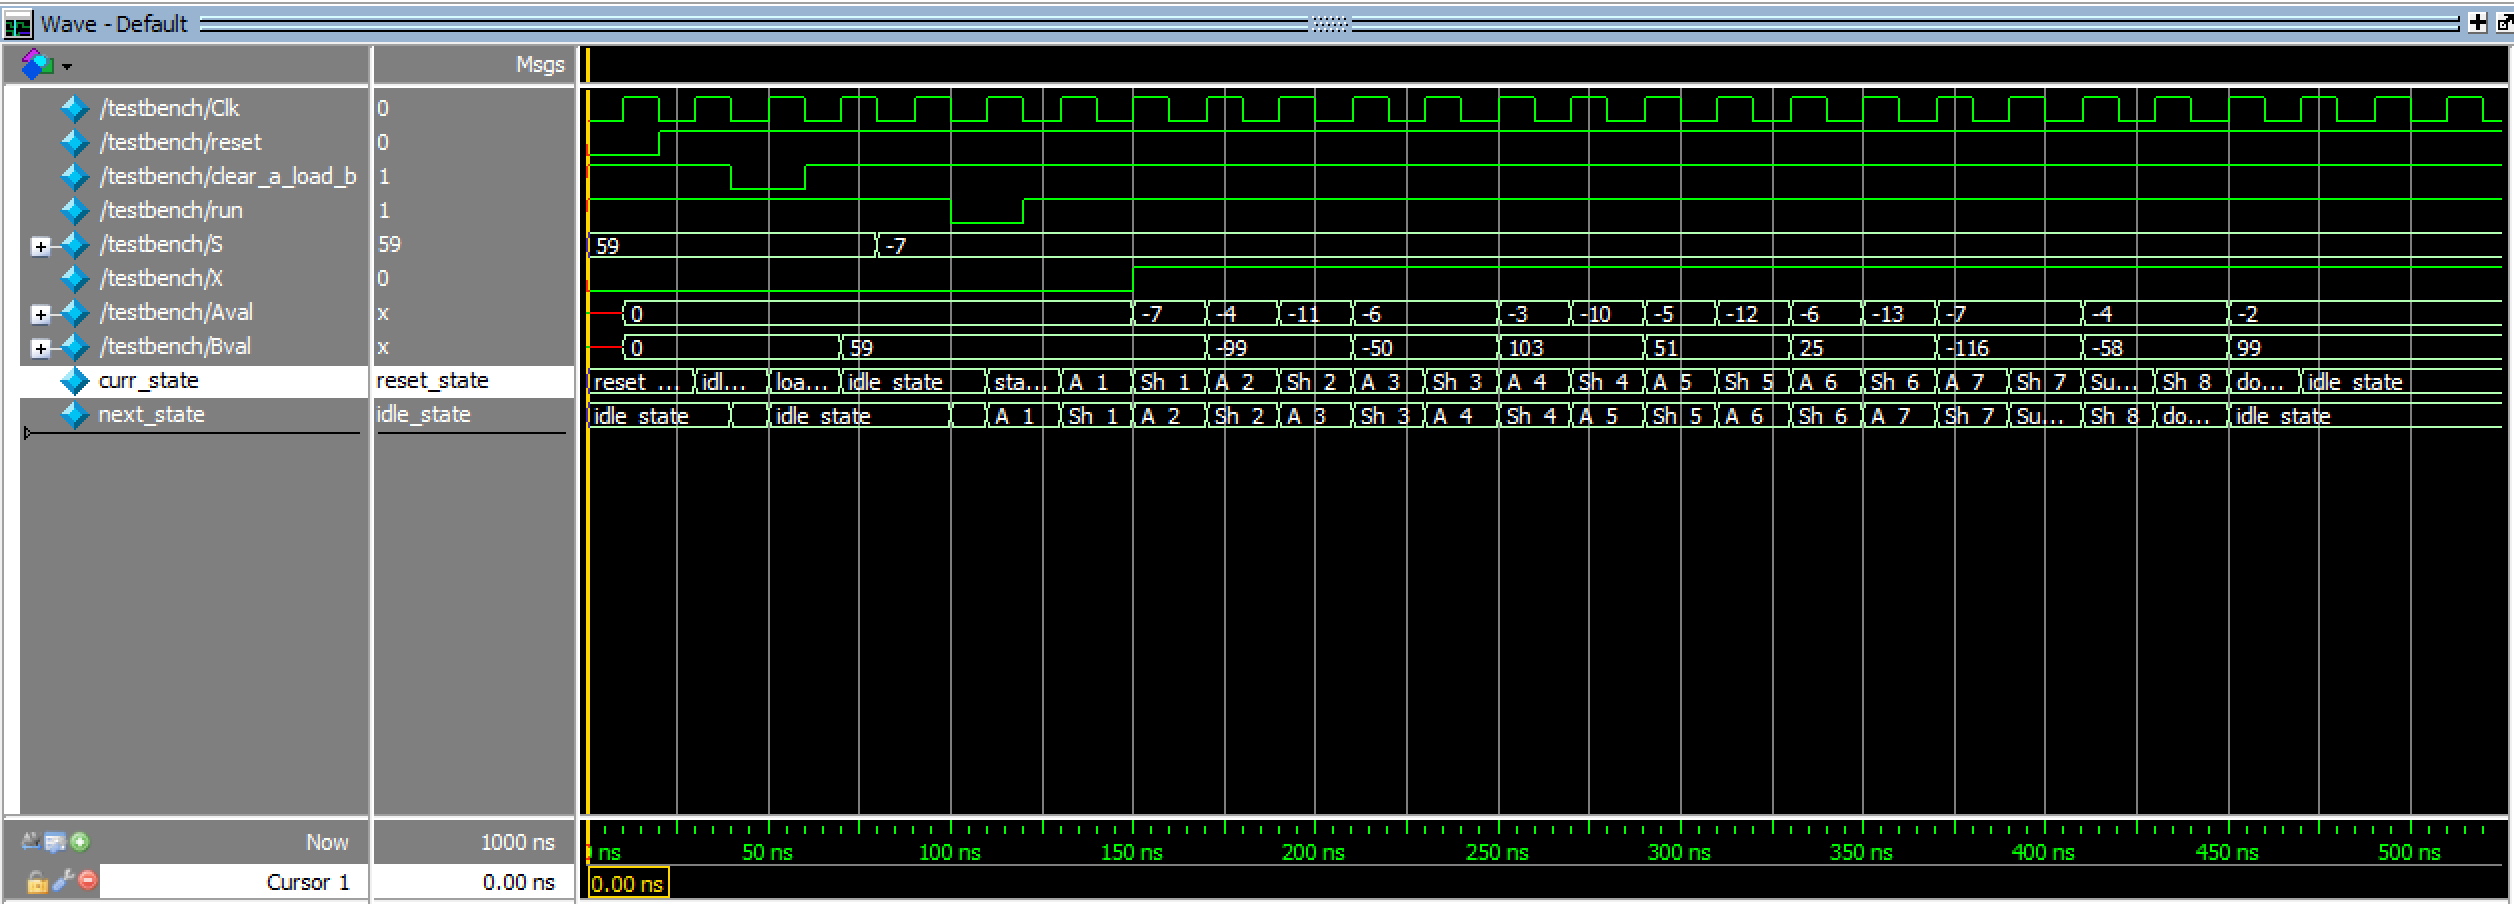
\includegraphics[scale=0.4]{simulation2.png}
	\caption{ModelSim Simulation Output (-7 * +59)\label{fig:simulation2t}}
\end{figure}

\begin{figure} [htbp]
	\centering
	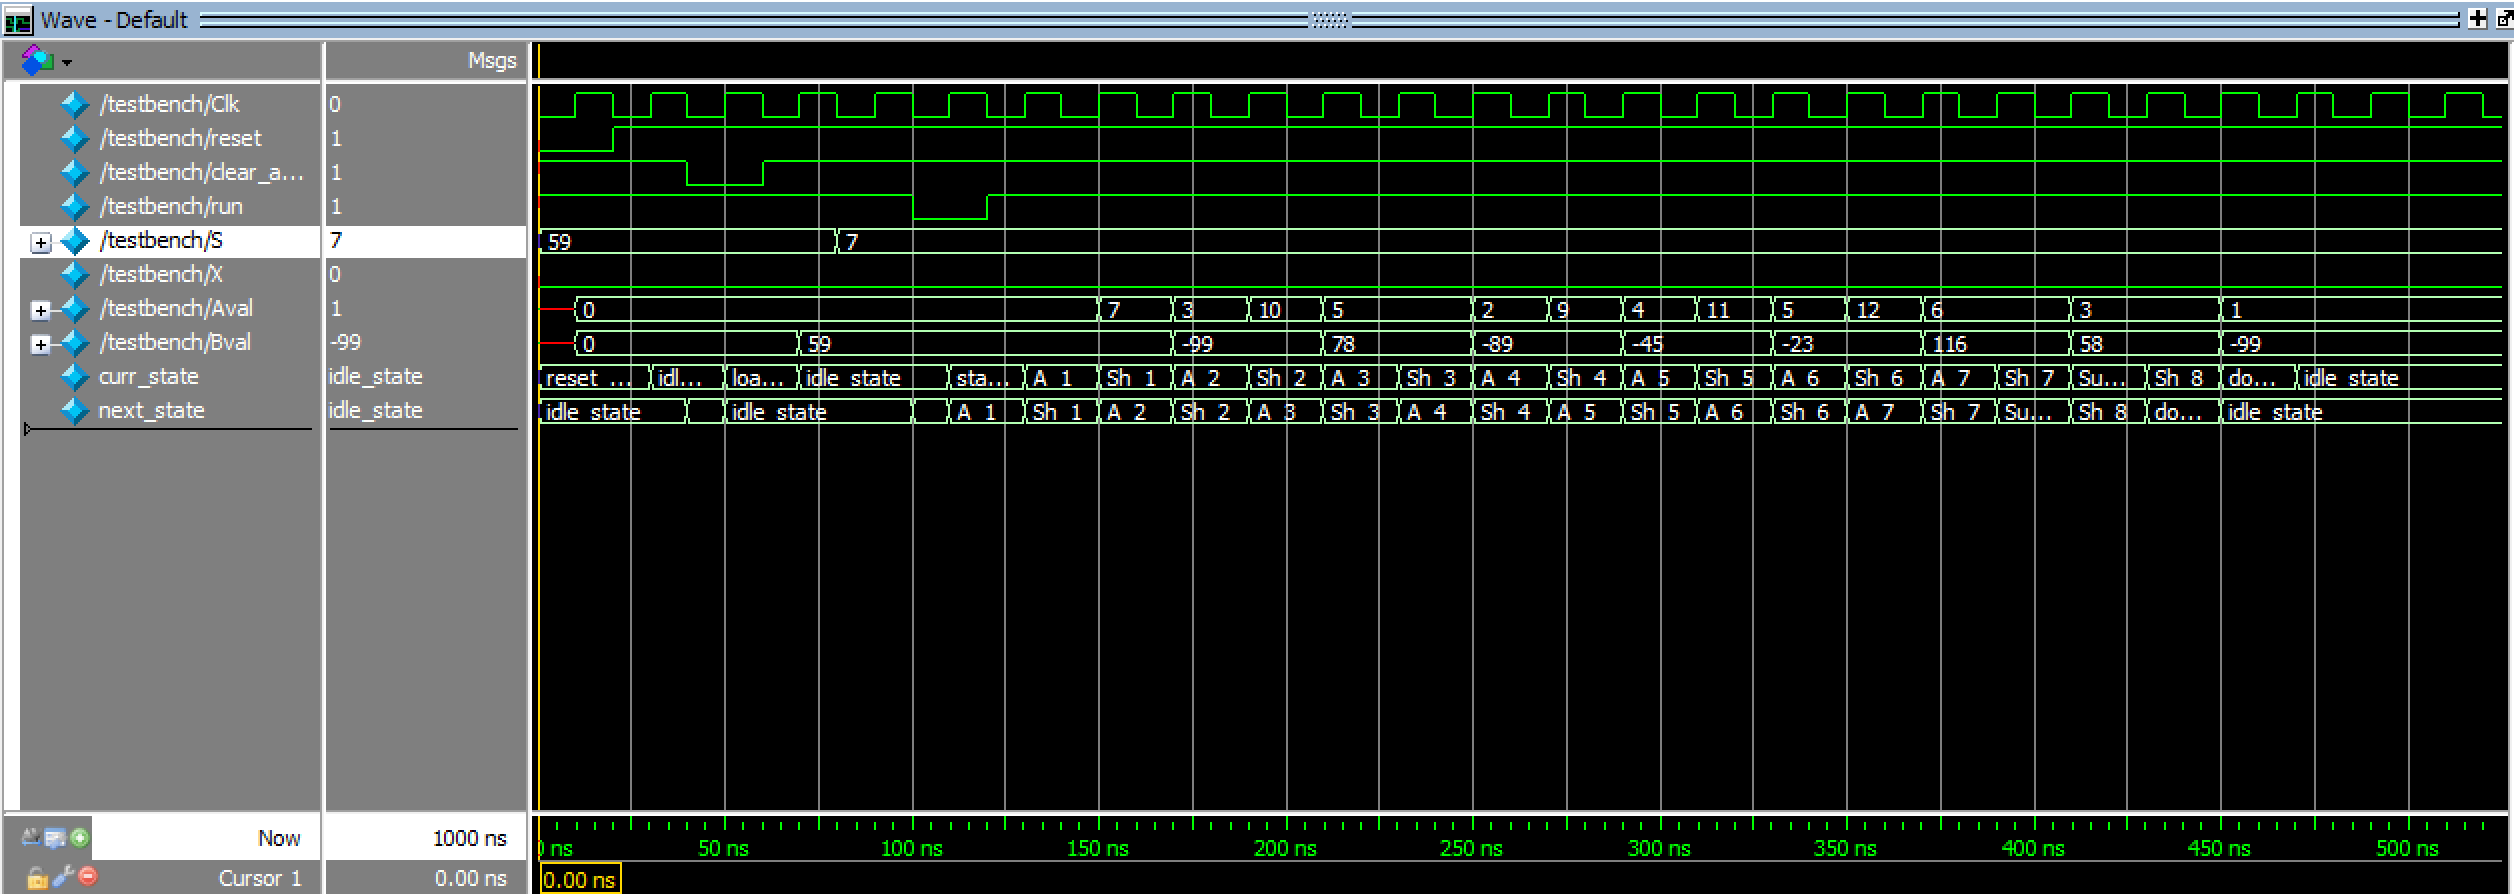
\includegraphics[scale=0.4]{simulation3.png}
	\caption{ModelSim Simulation Output (+7 * +59)\label{fig:simulation3}}
\end{figure}

\begin{figure} [htbp]
	\centering
	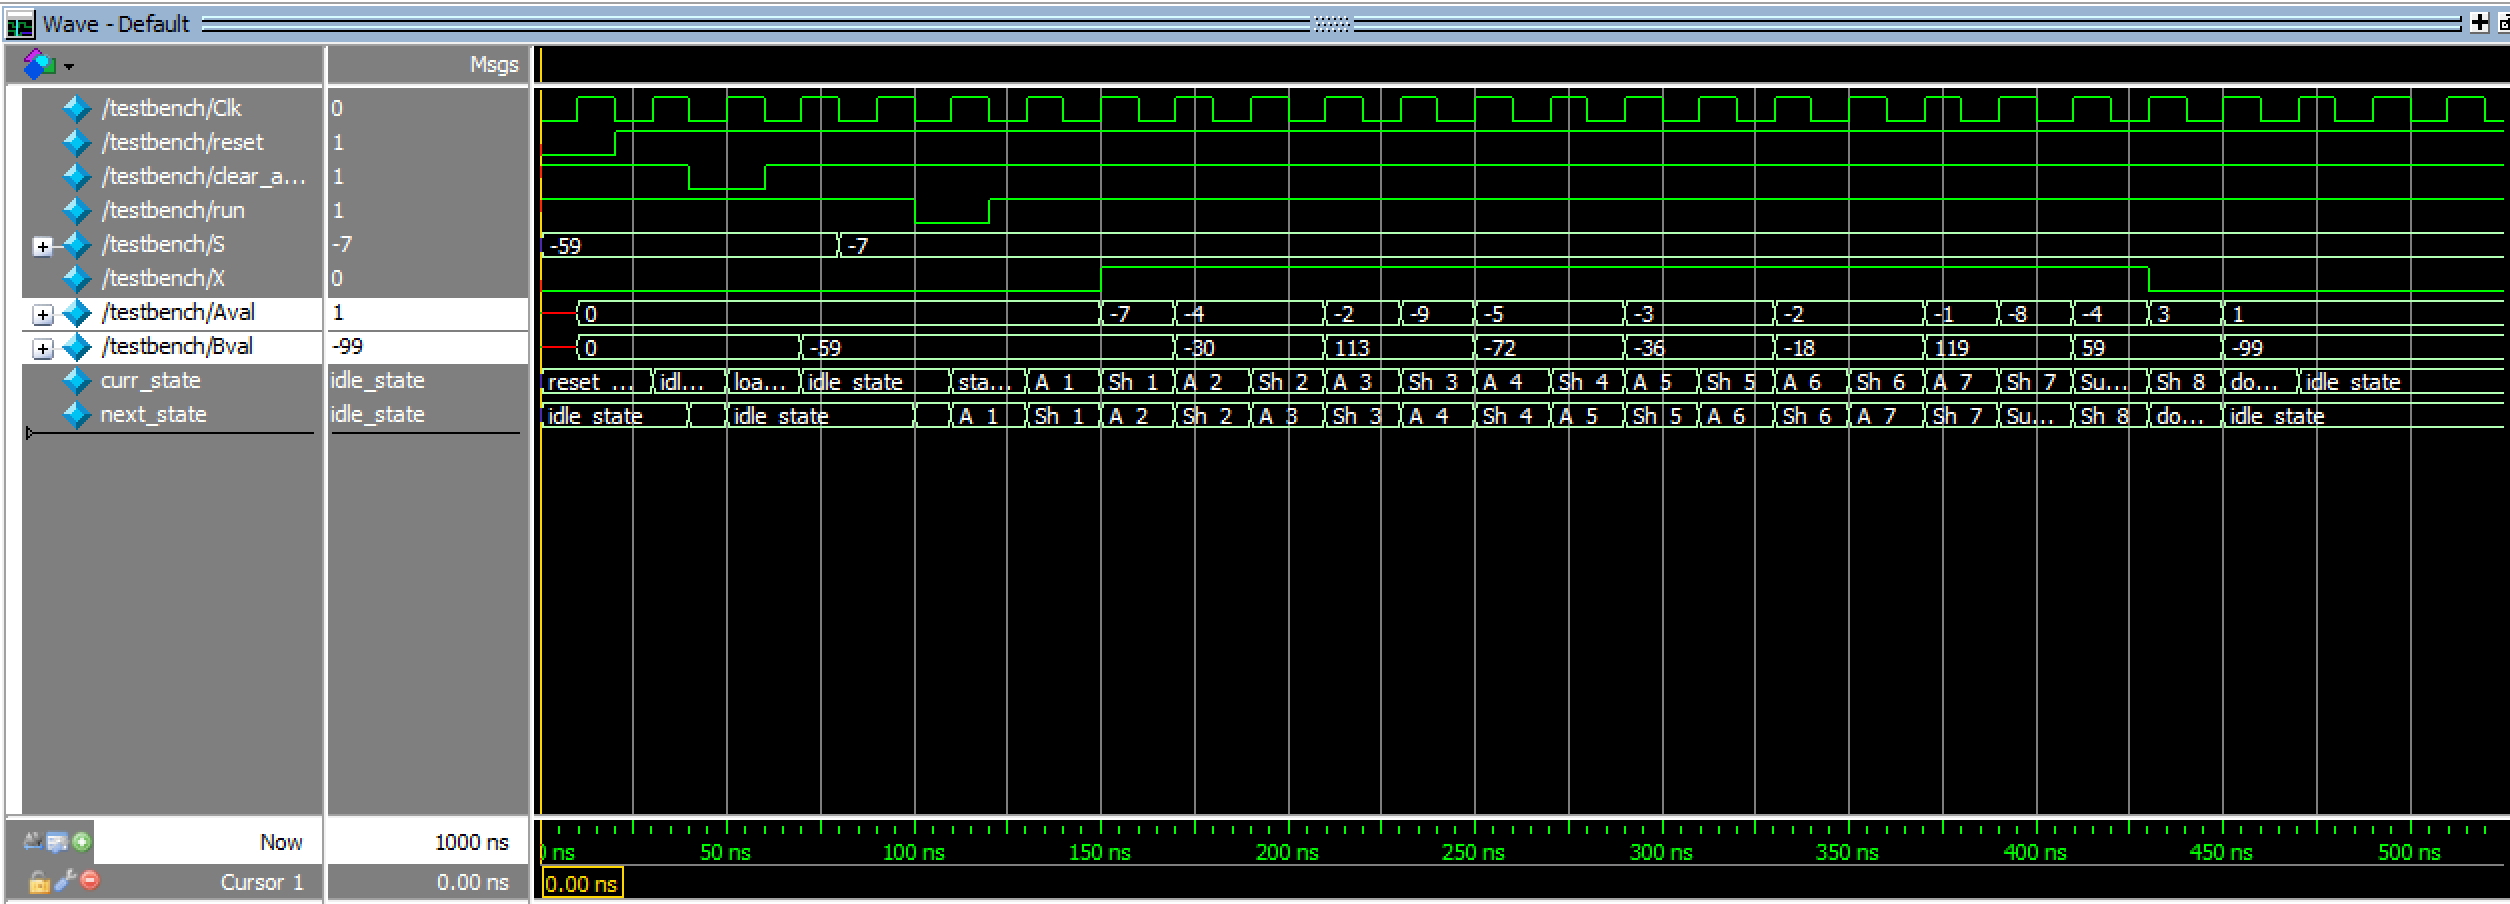
\includegraphics[scale=0.4]{simulation4.png}
	\caption{ModelSim Simulation Output (-7 * -59)\label{fig:simulation4}}
\end{figure}

\begin{figure} [htbp]
	\centering
	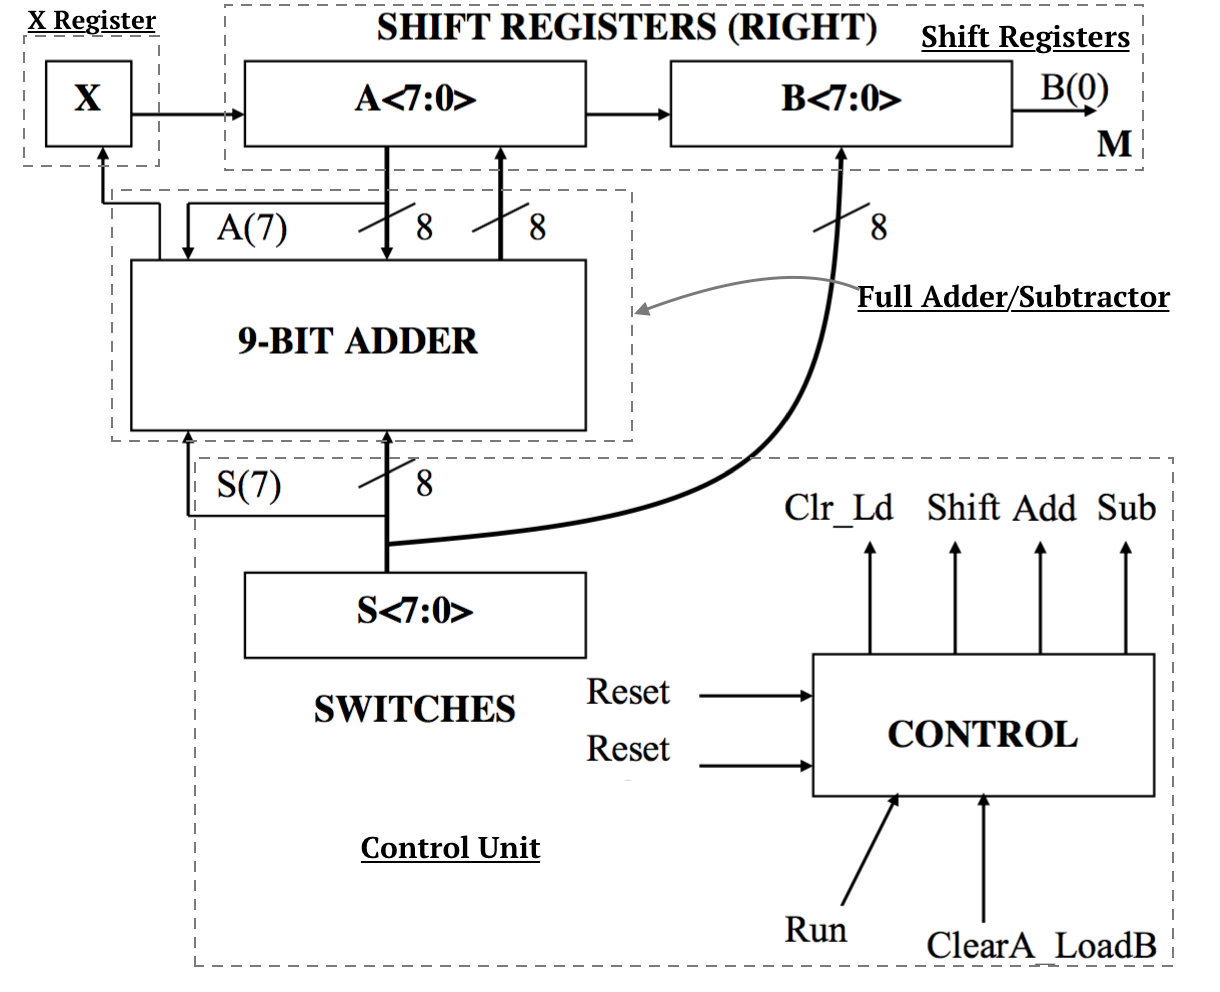
\includegraphics[scale=0.6]{Block_Diagram.png}
	\caption{Incomplete Module Block Diagram\label{fig:block-diagram}}
\end{figure}

\begin{figure} [htbp]
	\centering
	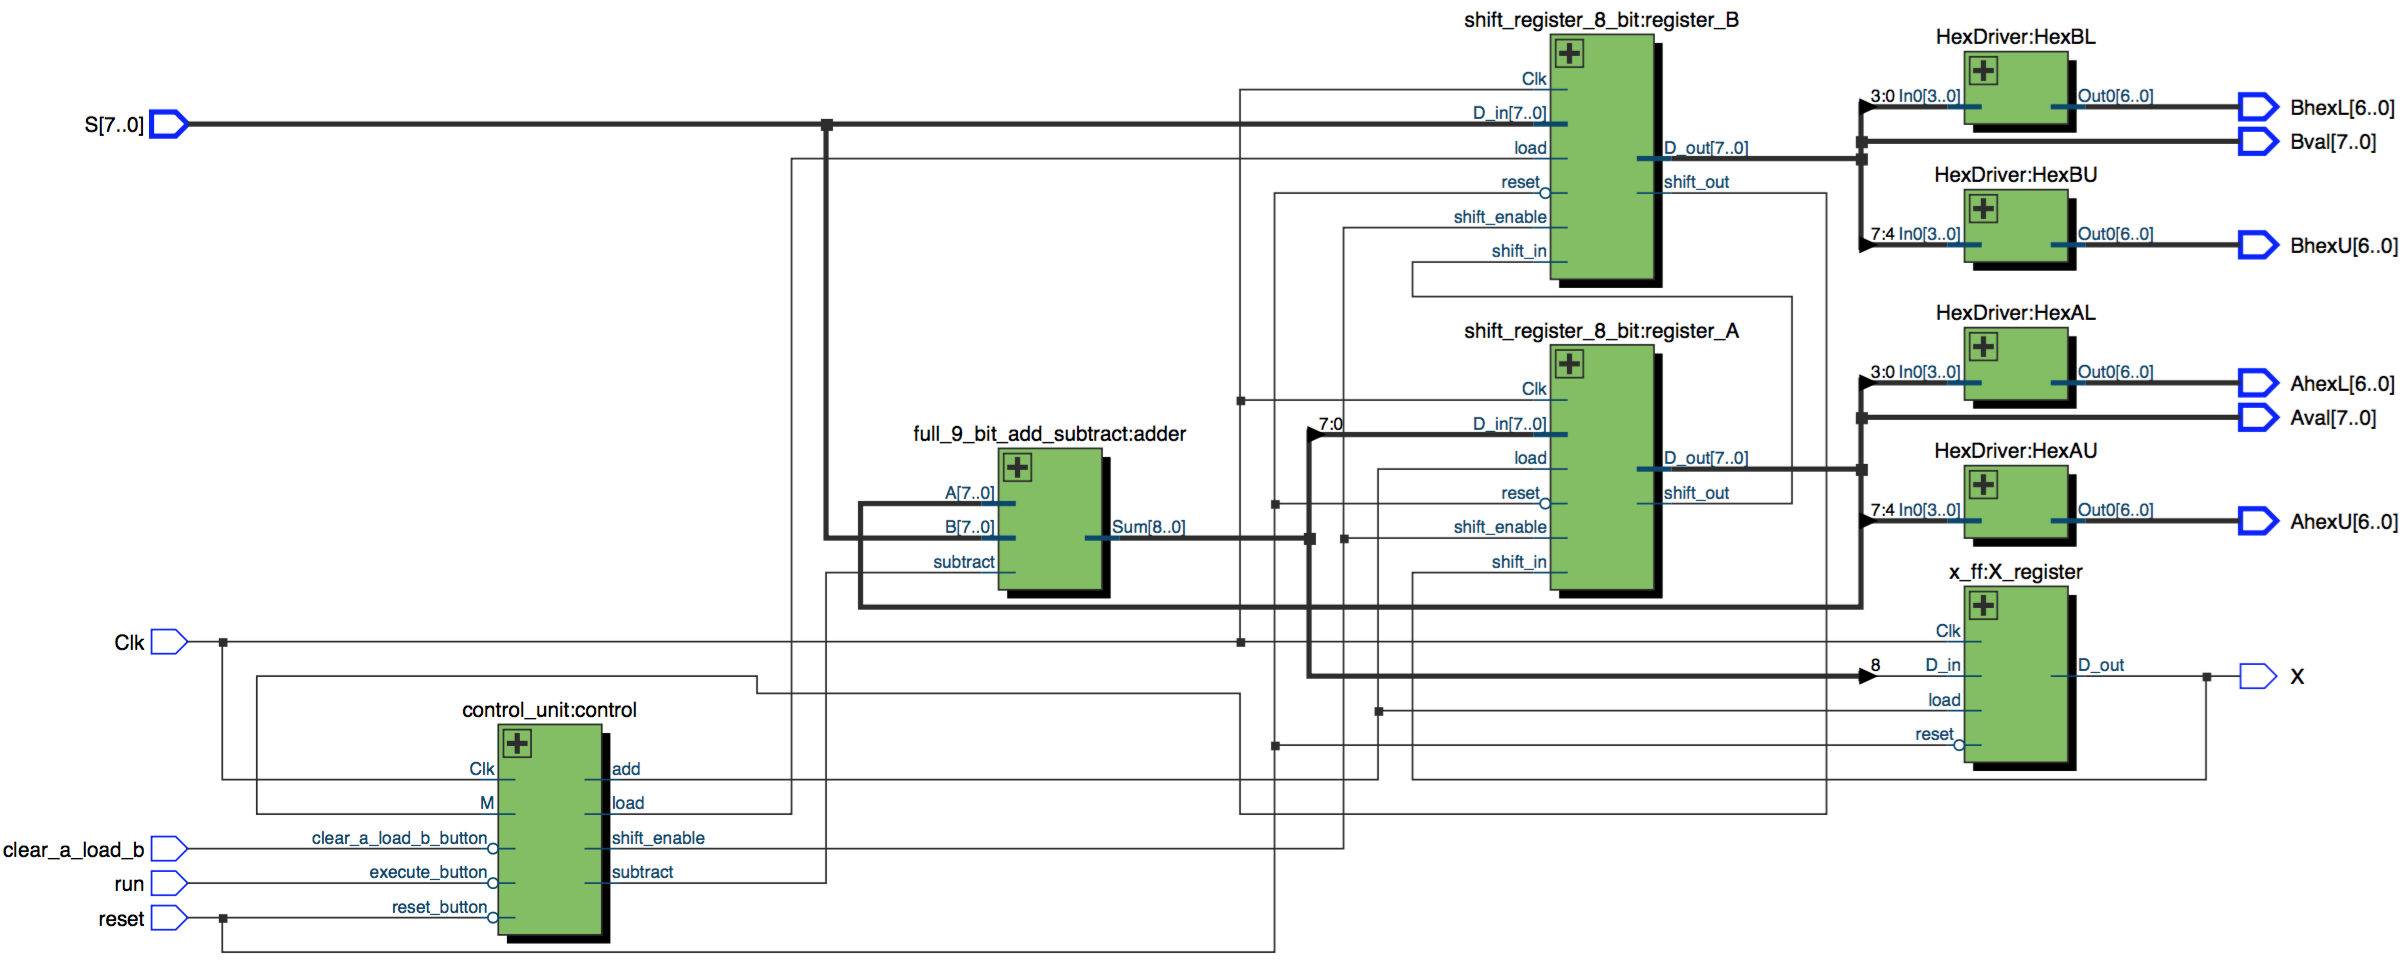
\includegraphics[scale=0.4]{full-multiplier-diagram.png}
	\caption{Full Multiplier Block Diagram\label{fig:full-multiplier-diagram}}
\end{figure}

\begin{figure} [htbp]
	\centering
	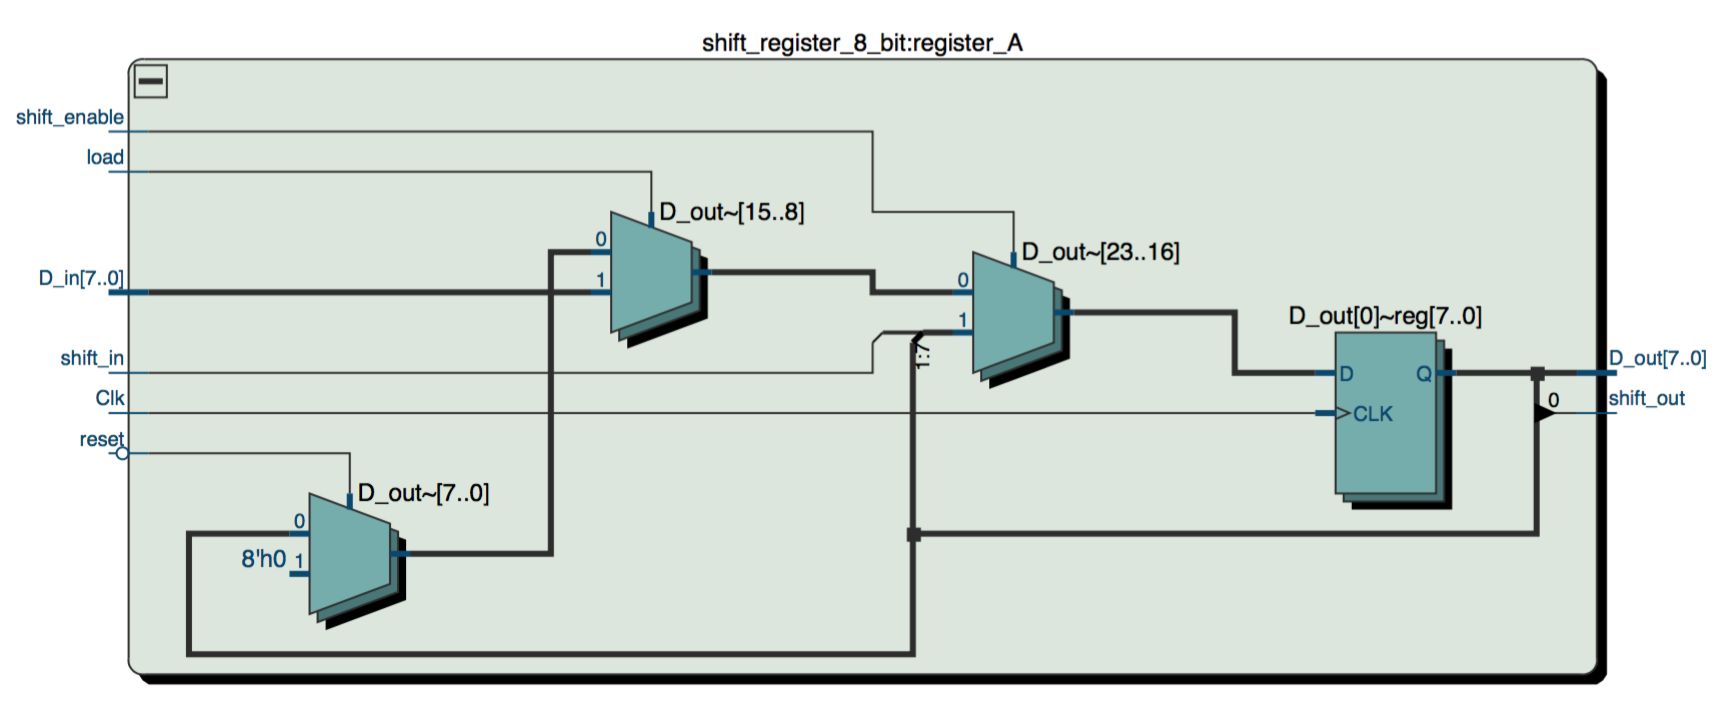
\includegraphics[scale=0.5]{shift-register-diagram.png}
	\caption{Shift Register Block Diagram\label{fig:shift-register-diagram}}
\end{figure}

\begin{figure} [htbp]
	\centering
	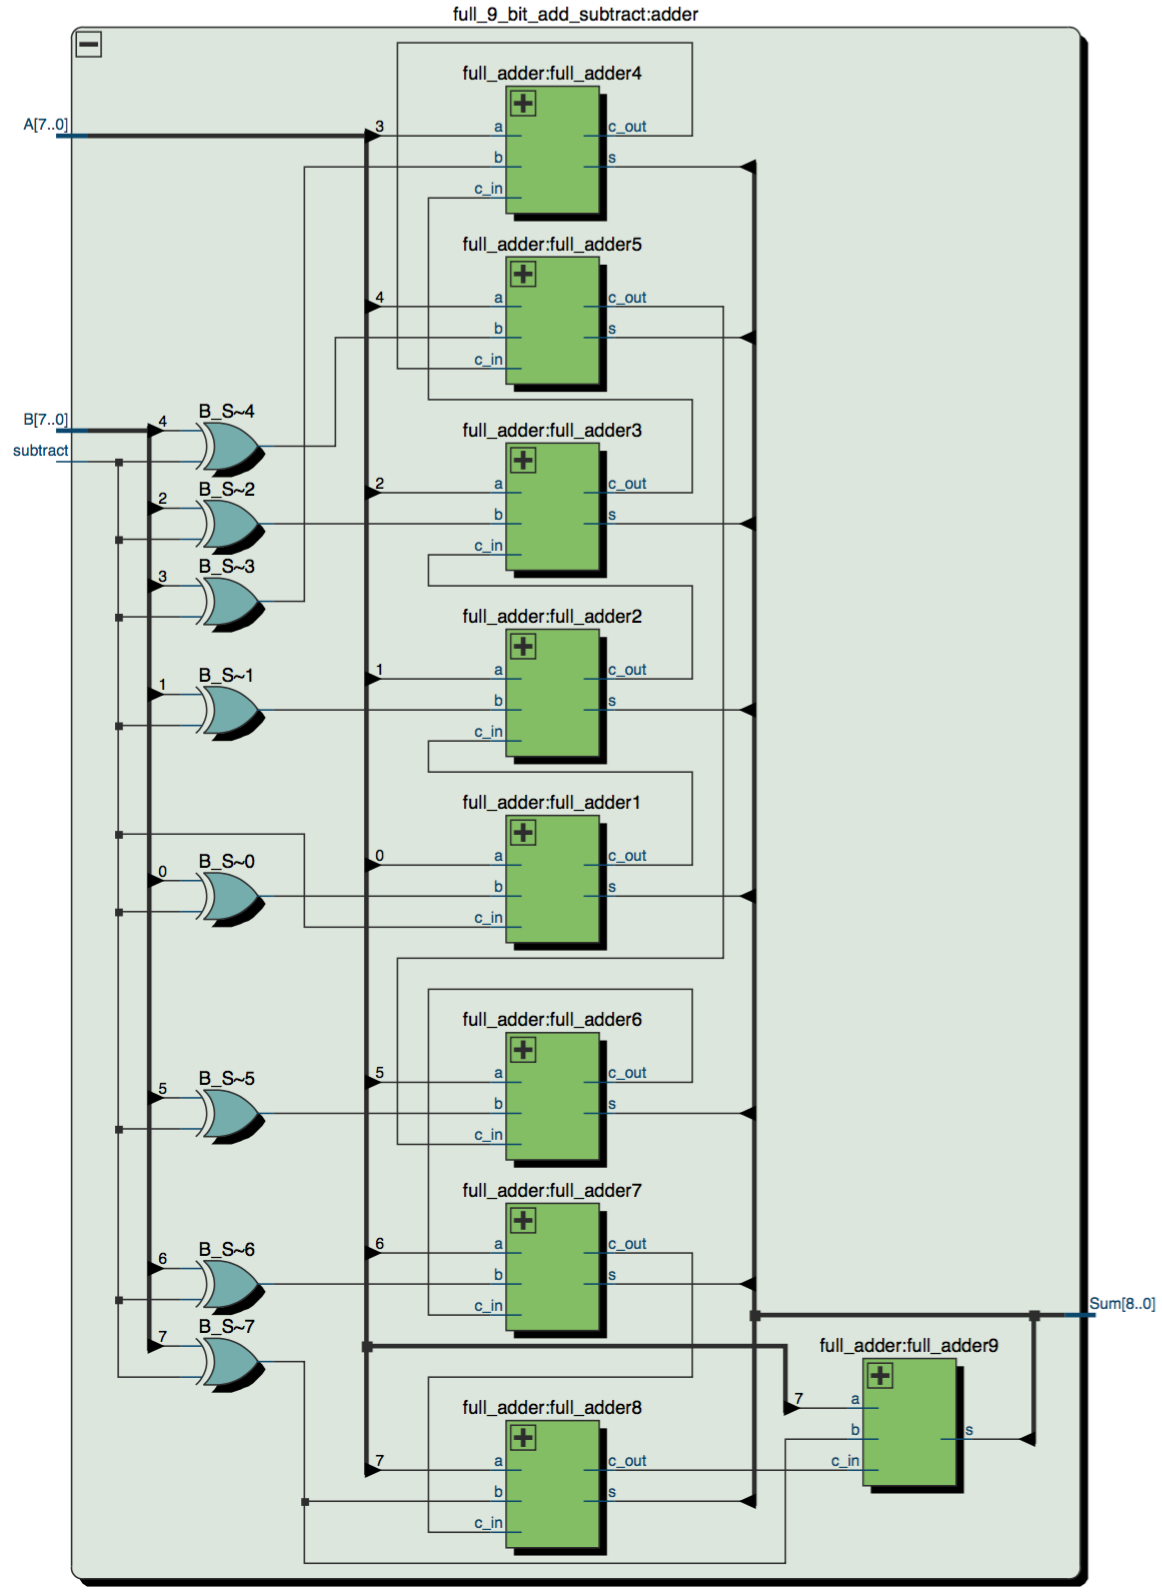
\includegraphics[scale=0.5]{full-adder-subtractor-diagram.png}
	\caption{Full Adder and Subtractor Block Diagram\label{fig:full-adder-subtractor-diagram}}
\end{figure}

\begin{figure} [htbp]
	\centering
	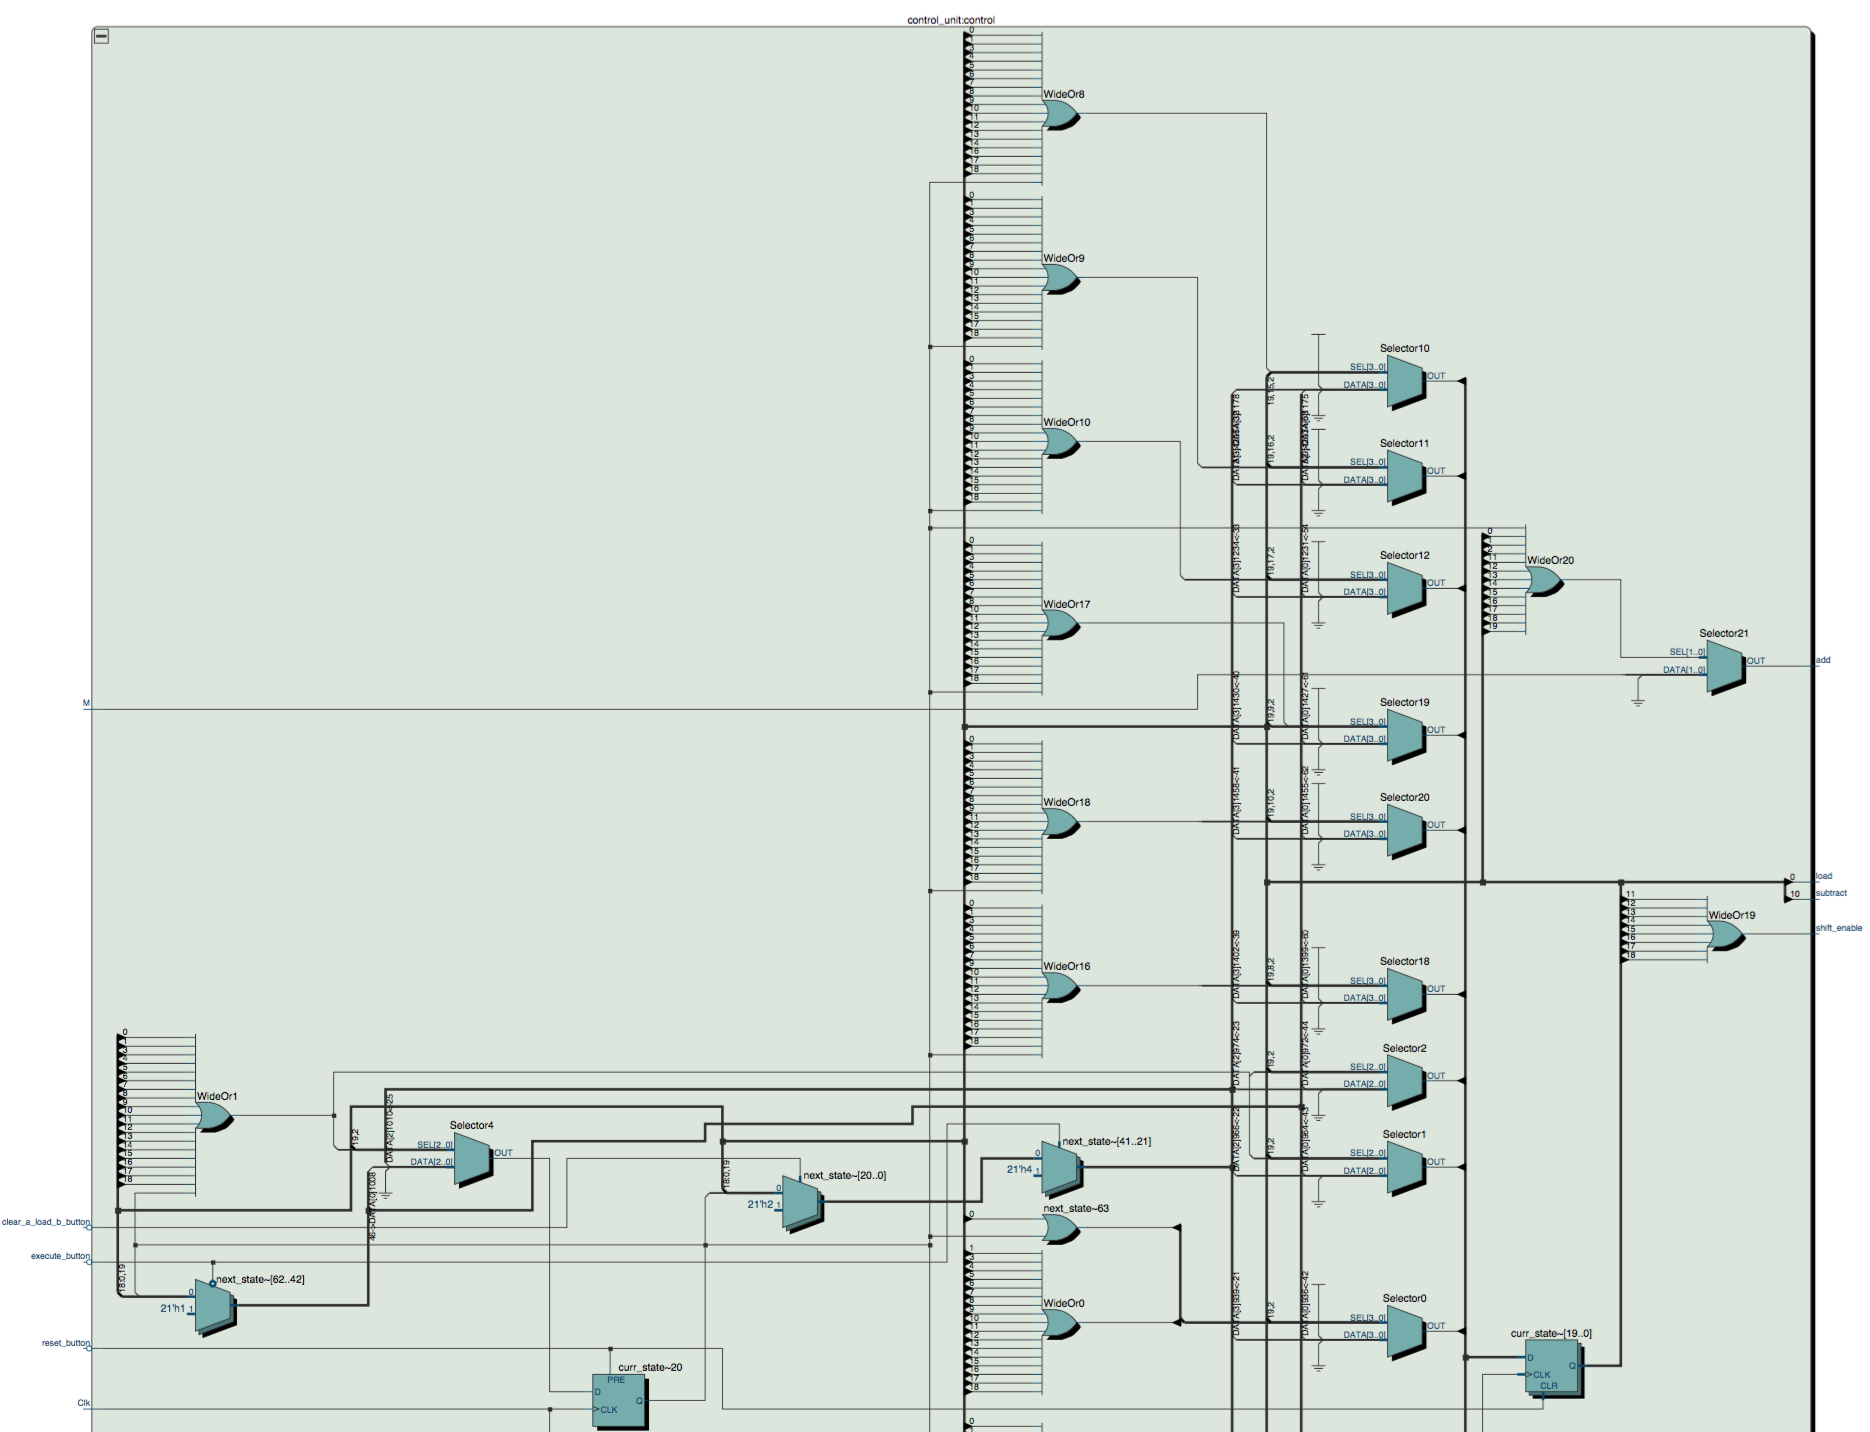
\includegraphics[scale=0.55]{control-unit-top-half-diagram.png}
		\caption{Top Half Control Unit Block Diagram\label{fig:top-half-control}}
\end{figure}

\begin{figure} [htbp]
	\centering
	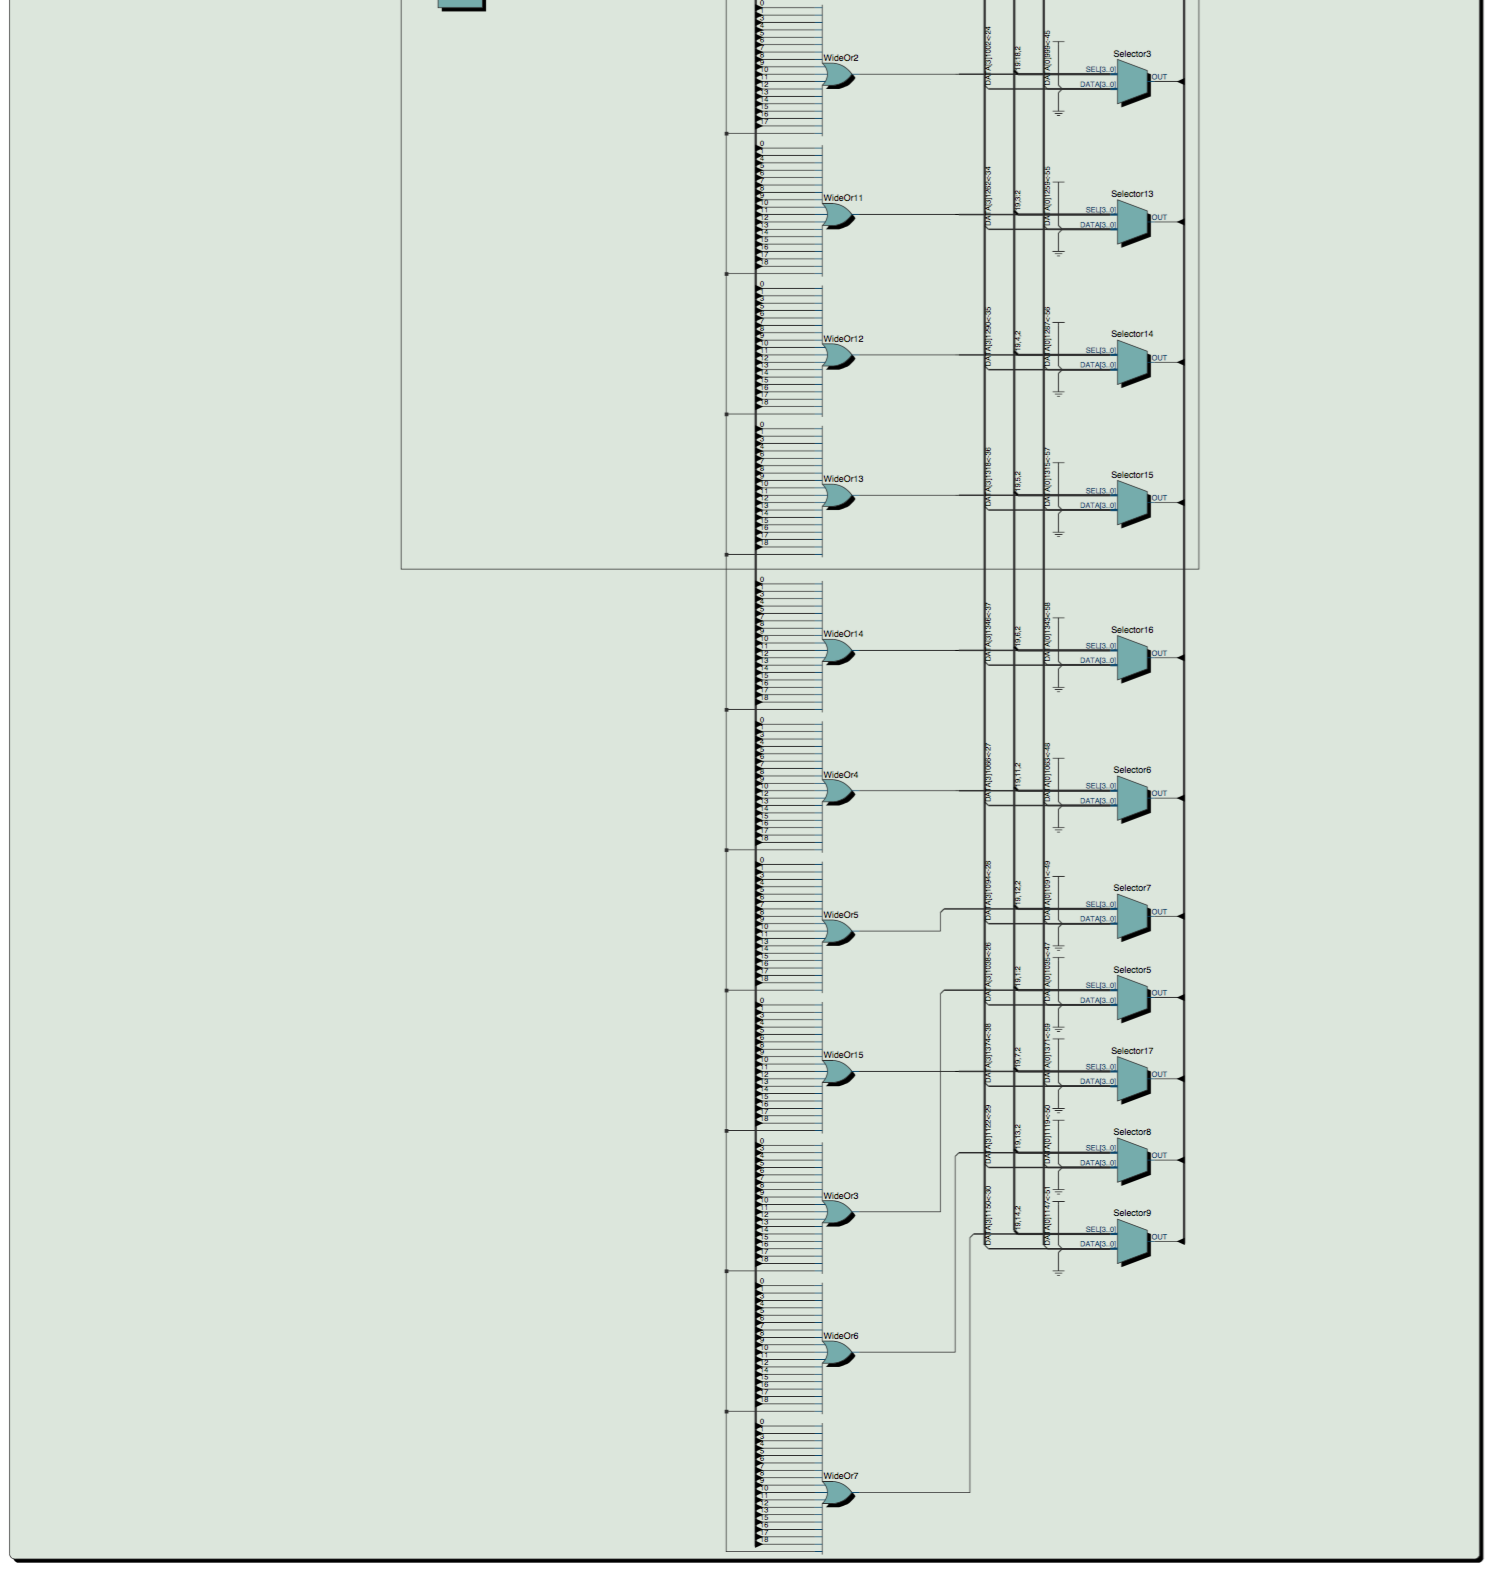
\includegraphics[scale=0.65]{control-unit-bottom-half-diagram.png}
	\caption{Bottom Half Control Unit Block Diagram\label{fig:bottom-half-control}}
\end{figure}

\begin{figure} [htbp]
	\centering
	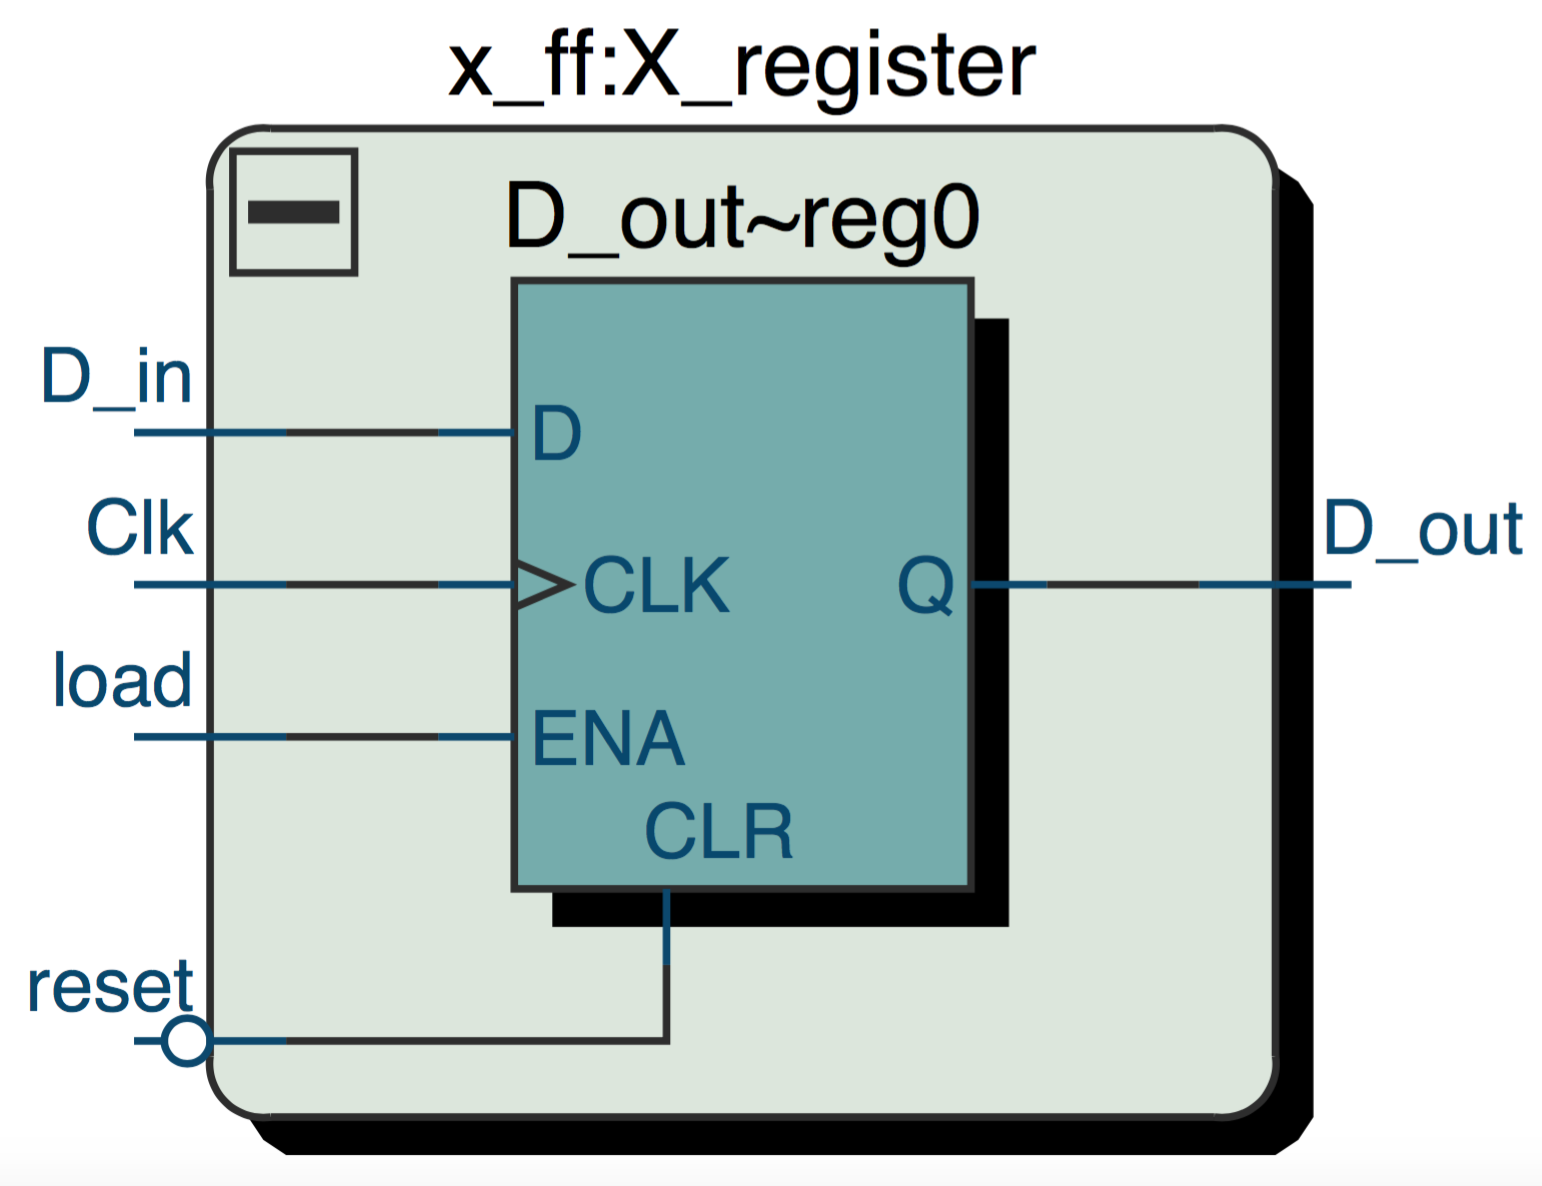
\includegraphics[scale=0.4]{x-ff-diagram.png}
	\caption{X-Bit Flip Flop Block Diagram\label{fig:x-ff-diagram}}
\end{figure}





%SECTION : Bibliography
%Insert Bibliography if needed

\end{document}